% Compile with XeLaTeX (twice) or Tectonic. All diagrams are embedded TikZ.
\documentclass[11pt,a4paper]{report}
\usepackage[margin=24mm,headheight=15pt]{geometry}
\usepackage{fontspec}
\setmainfont{lmroman10-regular.otf}[BoldFont=lmroman10-bold.otf,ItalicFont=lmroman10-italic.otf,BoldItalicFont=lmroman10-bolditalic.otf]
\usepackage{microtype,graphicx,booktabs,tabularx,longtable,array,enumitem}
\usepackage{xcolor,tikz,fancyhdr,titlesec,float}
\usetikzlibrary{arrows.meta,positioning,shapes.geometric,fit,calc}
\usepackage[colorlinks=true,linkcolor=black,urlcolor=blue]{hyperref}
\definecolor{ink}{HTML}{183F36}
\definecolor{wash}{HTML}{EDF3F0}
\pagestyle{fancy}\fancyhf{}\fancyhead[L]{\small UCS503 -- Software Engineering Lab}\fancyhead[R]{\small Campus Reserve}\fancyfoot[C]{\thepage}
\titleformat{\chapter}[display]{\bfseries\Large}{Chapter \thechapter}{8pt}{\huge}
\titlespacing*{\chapter}{0pt}{0pt}{20pt}
\setlength{\parindent}{0pt}\setlength{\parskip}{6pt}
\setlist{nosep,leftmargin=18pt}\renewcommand{\arraystretch}{1.25}
\newcolumntype{Y}{>{\raggedright\arraybackslash}X}
\tikzset{box/.style={draw=ink,rounded corners=2pt,fill=wash,align=center,font=\small,text width=3.2cm,minimum height=10mm}, actor/.style={draw,align=center,font=\small,minimum width=2.5cm,minimum height=9mm},arr/.style={-{Latex[length=2mm]},thick,draw=ink},decision/.style={diamond,aspect=2.4,draw=ink,fill=wash,align=center,font=\small,inner sep=2pt}}
\newcommand{\src}[1]{\nolinkurl{#1}}
\newcommand{\uc}[6]{\subsection{#1}\begin{tabularx}{\textwidth}{@{}p{30mm}Y@{}}\toprule Actor & #2\\ Preconditions & #3\\ Main flow & #4\\ Alternate flow & #5\\ Postcondition & #6\\\bottomrule\end{tabularx}}
\begin{document}
\begin{titlepage}\centering
\vspace*{15mm}{\Large\bfseries UCS503 -- Software Engineering Lab\par}
\vspace{16mm}{\Huge\bfseries Campus Resource\par Management System\par}
\vspace{5mm}{\Large Campus Reserve\par}
\vspace{4mm}{\large Software Engineering Prototype Report\par}
\vspace{17mm}{\large\bfseries Submitted by\par}\vspace{4mm}
\begin{tabular}{ll}Aditya Bhardwaj & 1024030777\\Ayati Kalra & 1024030783\\Rishita Jain & 1024030782\end{tabular}
\vspace{7mm}\par Group: \rule{40mm}{0.4pt}
\vspace{15mm}\par{\large\bfseries Submitted to}\par\vspace{5mm}\rule{75mm}{0.4pt}
\vfill{\large Mid-Semester Evaluation\par}
\vspace{3mm}{\bfseries Computer Science and Engineering Department\par}
Thapar Institute of Engineering and Technology, Patiala\par
\vspace{6mm}{\small Repository-based prototype documentation\par September 2026}
\end{titlepage}
\pagenumbering{roman}\tableofcontents\clearpage
\chapter*{Abstract}\addcontentsline{toc}{chapter}{Abstract}
Campus Reserve is a campus resource booking prototype for student societies, permission in-charges and campus administrators. It brings room availability, reservation requests, review decisions and booking records into one browser interface. Students select a campus space and time, complete an eight-step request form, and track its status. Permission in-charges approve or reject requests, while administrators maintain room and society records.

The current implementation uses React, TypeScript and Vite, with browser localStorage for persistence. It demonstrates workflow and interface behaviour without a backend, shared database or production authentication. This report adapts the supplied UCS503 report's project-selection and analysis structure to the linked repository. It includes use-case specifications, activity and interaction models, a conceptual data model, data-flow diagrams, requirements, user stories and a prototype demonstration plan.

\textbf{Scope of evidence.} Descriptions derive from repository documentation and inspected source files on 15 September 2026. Diagram models describe or abstract the current implementation unless marked as proposed. No deployment, load benchmark or independent application test result is claimed. The reference report provides structure only; its health-chatbot content and contributor details do not apply to this project.
\clearpage\pagenumbering{arabic}
\chapter{Project Selection Phase}
\section{Software Bid}
Campus activities require suitable spaces and a clear permission process. A booking workflow spread across informal messages and separate records can make availability and approval status difficult to follow. This is the problem the project addresses; no survey or measured baseline is claimed.

The proposed campus portal provides a common interface for discovering rooms, submitting society requests and recording review decisions. Its prototype supports an academic demonstration of software analysis, interface design, validation and state management. The present scope focuses on rooms and campus spaces. Equipment requirements can be recorded within an activity request, but the repository does not implement a separate equipment inventory or lending system.
\section{Project Overview}
\begin{itemize}
\item Students and society representatives browse availability and submit reservation requests.
\item Permission in-charges review pending requests and record approval or rejection.
\item Administrators add or update room and society information.
\item Local notifications communicate booking submissions and status changes.
\item The browser preserves demo data through localStorage.
\end{itemize}
\section{Objectives and Boundaries}
\begin{tabularx}{\textwidth}{@{}YY@{}}\toprule Prototype objective & Current boundary\\\midrule Make availability visible & Data is local to one browser, not synchronized campus-wide.\\Prevent overlapping requests & Client-side checks compare Pending and Approved bookings.\\Demonstrate role-specific workflows & Demo persona switching does not verify passwords.\\Maintain booking history & Local records can be cleared or changed by the browser user.\\Capture permission decisions & No authoritative institutional approval integration exists.\\\bottomrule\end{tabularx}
\section{Proposed Completion Plan}
\begin{tabularx}{\textwidth}{@{}p{24mm}YY@{}}\toprule Stage & Work & Exit condition\\\midrule 1 & Review requirements and prototype & Faculty accepts scope and workflows.\\2 & Demonstrate booking and review paths & Core scenarios produce expected state changes.\\3 & Improve validation and access controls & Agreed acceptance criteria pass.\\4 & Introduce API and database & Shared persistence and server-side conflict control work.\\5 & Pilot and document & User feedback and test evidence support deployment.\\\bottomrule\end{tabularx}
This is a proposed next-stage plan, not a claim about completed milestones or a fixed semester schedule.
\chapter{Analysis Phase}
\section{Use Cases}
\subsection{Use-Case Diagram}
\begin{figure}[H]\centering
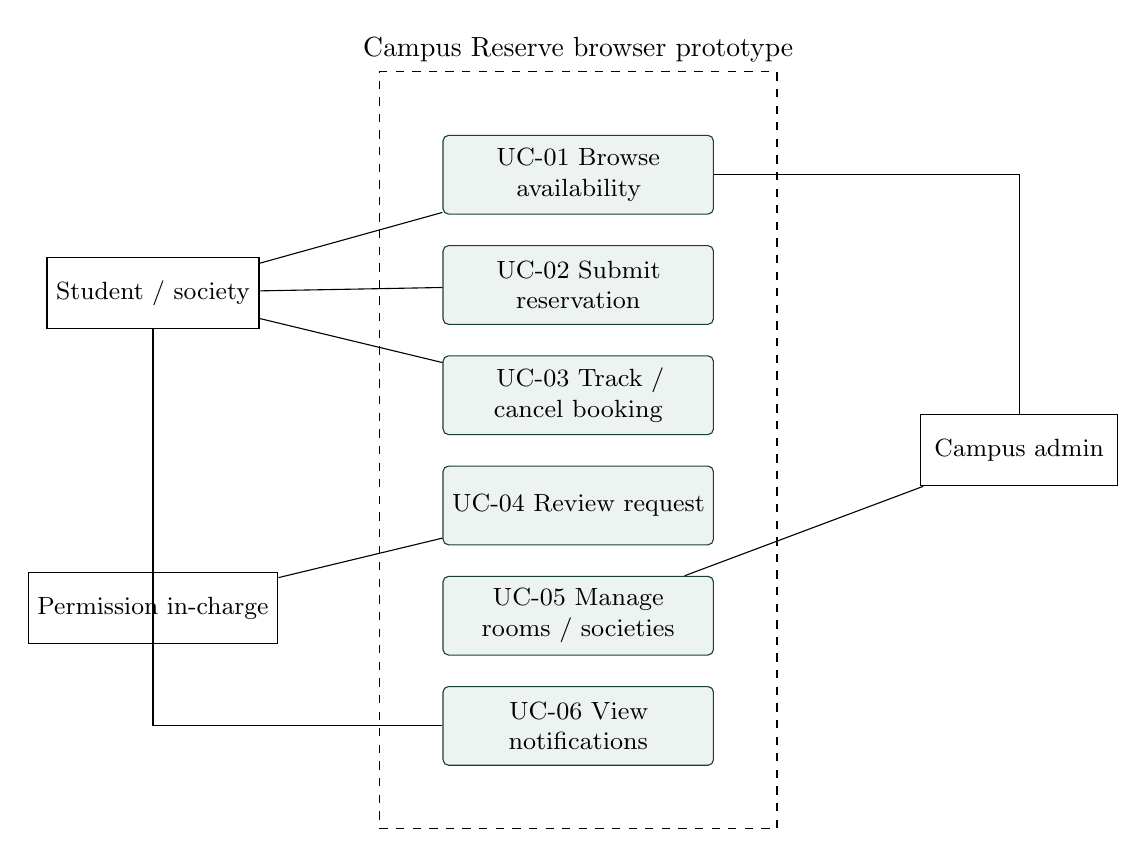
\begin{tikzpicture}[x=1cm,y=1cm]
\node[actor] (s) at (0,1.5) {Student / society};
\node[actor] (i) at (0,-2.5) {Permission in-charge};
\node[actor] (a) at (11,-0.5) {Campus admin};
\node[box] (u1) at (5.4,3) {UC-01 Browse availability};
\node[box] (u2) at (5.4,1.6) {UC-02 Submit reservation};
\node[box] (u3) at (5.4,0.2) {UC-03 Track / cancel booking};
\node[box] (u4) at (5.4,-1.2) {UC-04 Review request};
\node[box] (u5) at (5.4,-2.6) {UC-05 Manage rooms / societies};
\node[box] (u6) at (5.4,-4) {UC-06 View notifications};
\draw (s)--(u1);\draw (s)--(u2);\draw (s)--(u3);\draw (s.south) |- (u6.west);
\draw (i)--(u4);\draw (i.south) |- (u6.west);\draw (a)--(u5);\draw (a.north) |- (u1.east);
\node[draw,dashed,fit=(u1)(u6),inner sep=8mm,label=above:Campus Reserve browser prototype] {};
\end{tikzpicture}
\caption{Primary actor interactions. Shared availability is available across roles.}
\end{figure}
\textbf{Supporting functions:} form validation, overlap detection, local persistence and notification creation support these user goals. They are internal functions rather than separate human actors. Persona selection simulates role access for the demonstration.
\clearpage
\subsection{Use-Case Specifications}
\uc{UC-01: Browse Availability}{Student, permission in-charge or administrator}{The prototype has initialized room and booking data.}{Select location, room and date; inspect the hourly schedule; select an available slot to open the booking form with the room and time populated.}{Choose a different date, time or room if the displayed slot is blocked or unsuitable.}{The actor sees availability, or a student proceeds with a selected slot.}
\uc{UC-02: Submit Reservation}{Student / society representative}{A demo persona is active and a suitable room and society record exist.}{Choose activity, society, location and room; enter date and time; choose permission type; complete activity details; review and submit.}{Invalid dates, reversed times, unavailable rooms, conflicts or missing required details require correction. An end time after 20:00 requires Night Permission.}{The prototype stores a Pending booking with an identifier and creates an in-charge notification.}
\uc{UC-03: Track or Cancel Booking}{Student / society representative}{The browser contains booking records visible in the student's booking screen.}{Open My Bookings; search or filter by status; inspect details; use the available cancellation action and confirm.}{Cancel the confirmation dialog to leave the record unchanged. Records already in terminal states may not offer cancellation in the interface.}{The actor sees the current status; a confirmed cancellation records Cancelled and creates a notification.}
\clearpage
\uc{UC-04: Review Request}{Permission in-charge}{A Pending request exists in the local browser data.}{Open the pending queue; inspect activity and timing details; approve with optional remarks or reject with a reason; review the updated status.}{Close the dialog without deciding, or correct missing decision information requested by the interface.}{The booking becomes Approved or Rejected, review metadata is stored, and the prototype creates a student notification.}
\uc{UC-05: Manage Rooms and Societies}{Campus administrator}{An admin demo persona is active.}{Open Rooms or Societies; add or edit the selected record; save the changes; inspect the updated list.}{Correct invalid or incomplete form entries, or dismiss the form without saving.}{The local room or society collection reflects the saved changes.}
\uc{UC-06: View Notifications}{Student or permission in-charge}{Local notifications exist for booking activity.}{Open the notification panel or page; inspect messages; mark a notification or all notifications as read.}{An empty list or a list of already-read messages requires no action.}{Read-state changes persist in the browser. Notification routing uses recipient roles rather than verified individual recipients.}
\section{Business Rules}
\begin{enumerate}
\item A reservation contains a society, campus room, date, start time, end time, activity and permission type.
\item New reservations have status Pending. Approval, rejection and cancellation update that stored status.
\item Pending and Approved reservations block overlapping intervals for the same room and date. Rejected and Cancelled reservations do not.
\item Adjacent intervals are allowed. A booking ending at 11:00 does not conflict with a booking starting at 11:00.
\item End time must follow start time; the form rejects past dates and rooms marked Unavailable.
\item In the current form, an end time later than 20:00 requires Night Permission.
\end{enumerate}
\clearpage
\section{Activity and Swimlane Diagrams}
\subsection{Activity Diagram: Reservation Submission}
\begin{figure}[H]\centering
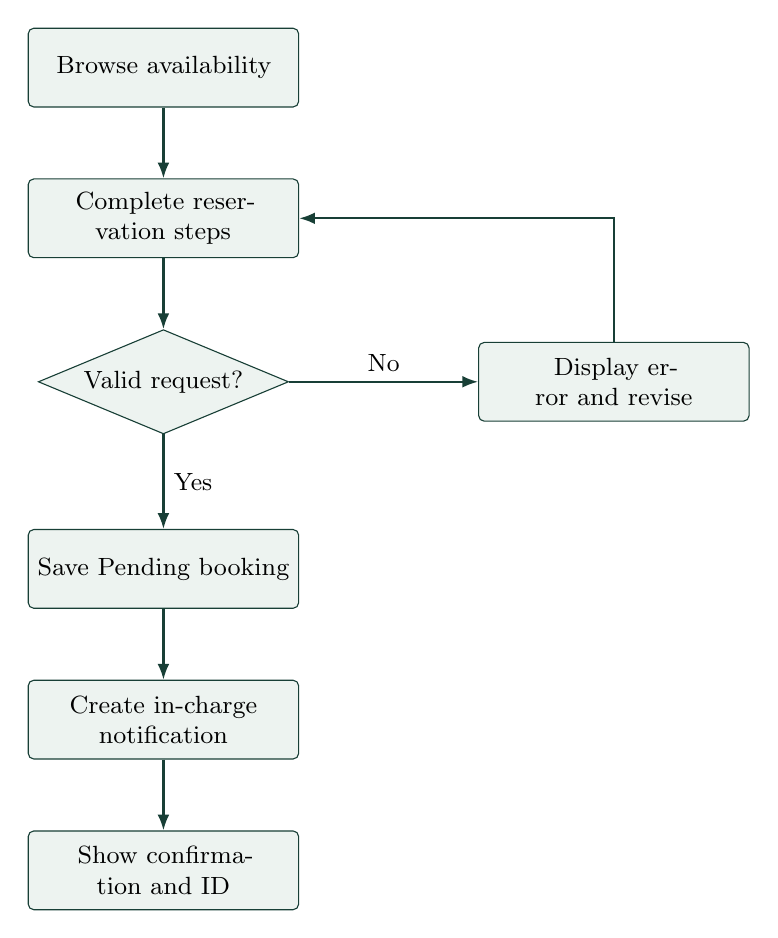
\begin{tikzpicture}[node distance=9mm]
\node[box] (b) {Browse availability};
\node[box,below=of b] (f) {Complete reservation steps};
\node[decision,below=of f] (v) {Valid request?};
\node[box,right=24mm of v] (e) {Display error and revise};
\node[box,below=12mm of v] (p) {Save Pending booking};
\node[box,below=of p] (n) {Create in-charge notification};
\node[box,below=of n] (c) {Show confirmation and ID};
\draw[arr] (b)--(f);\draw[arr](f)--(v);\draw[arr](v)--node[above,font=\small]{No}(e);
\draw[arr](e.north)|-(f.east);\draw[arr](v)--node[right,font=\small]{Yes}(p);
\draw[arr](p)--(n);\draw[arr](n)--(c);
\end{tikzpicture}\caption{Form checks precede a local booking write.}
\end{figure}
\subsection{Swimlane Diagram: Request to Decision}
\begin{figure}[H]\centering
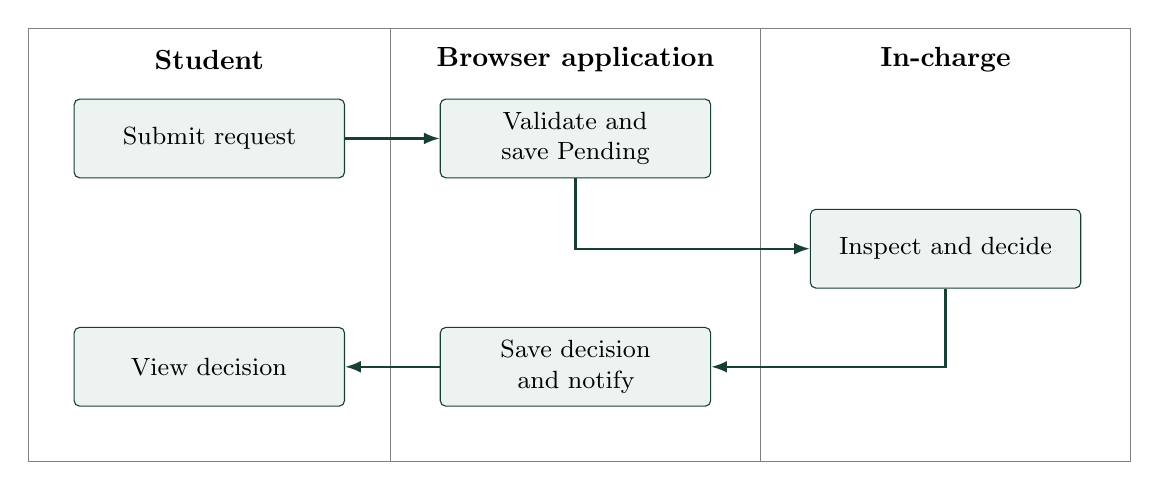
\begin{tikzpicture}[x=1cm,y=1cm]
\draw[gray] (0,0) rectangle (14,-5.5);\draw[gray](4.6,0)--(4.6,-5.5);\draw[gray](9.3,0)--(9.3,-5.5);
\node at (2.3,-.4){\textbf{Student}};\node at (6.95,-.4){\textbf{Browser application}};\node at (11.65,-.4){\textbf{In-charge}};
\node[box] (a) at (2.3,-1.4){Submit request};\node[box](b)at(6.95,-1.4){Validate and save Pending};
\node[box](c)at(11.65,-2.8){Inspect and decide};\node[box](d)at(6.95,-4.3){Save decision and notify};\node[box](e)at(2.3,-4.3){View decision};
\draw[arr](a)--(b);\draw[arr](b.south)|-(c.west);\draw[arr](c.south)|-(d.east);\draw[arr](d)--(e);
\end{tikzpicture}\caption{Role responsibilities. Persona switching occurs within the same browser demo.}
\end{figure}
\clearpage
\section{Sequence and Collaboration Diagrams}
\subsection{Sequence Diagram: Submit a Booking}
\begin{figure}[H]\centering
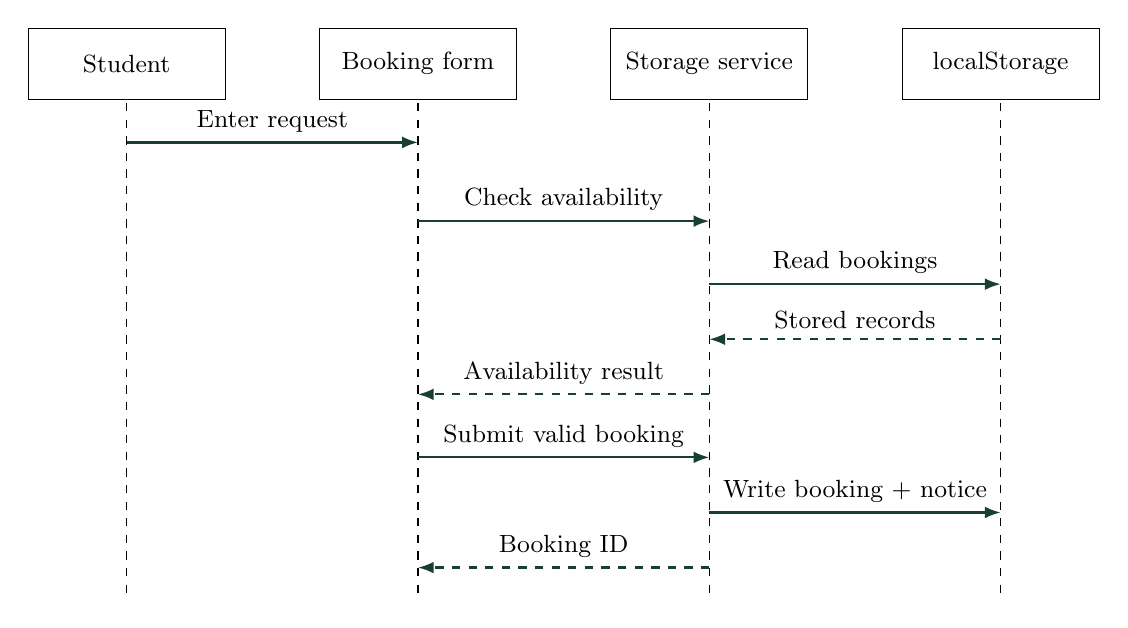
\begin{tikzpicture}[x=1cm,y=1cm,font=\small]
\foreach \x/\n in {0/Student,3.7/Booking form,7.4/Storage service,11.1/localStorage}{\node[actor] at (\x,0){\n};\draw[dashed](\x,-.5)--(\x,-6.8);}
\draw[arr](0,-1)--node[above]{Enter request}(3.7,-1);
\draw[arr](3.7,-2)--node[above]{Check availability}(7.4,-2);
\draw[arr](7.4,-2.8)--node[above]{Read bookings}(11.1,-2.8);
\draw[arr,dashed](11.1,-3.5)--node[above]{Stored records}(7.4,-3.5);
\draw[arr,dashed](7.4,-4.2)--node[above]{Availability result}(3.7,-4.2);
\draw[arr](3.7,-5)--node[above]{Submit valid booking}(7.4,-5);
\draw[arr](7.4,-5.7)--node[above]{Write booking + notice}(11.1,-5.7);
\draw[arr,dashed](7.4,-6.4)--node[above]{Booking ID}(3.7,-6.4);
\end{tikzpicture}\caption{Successful submission path. Invalid requests stay in the form for correction.}
\end{figure}
\subsection{Collaboration Diagram: Review a Request}
\begin{figure}[H]\centering
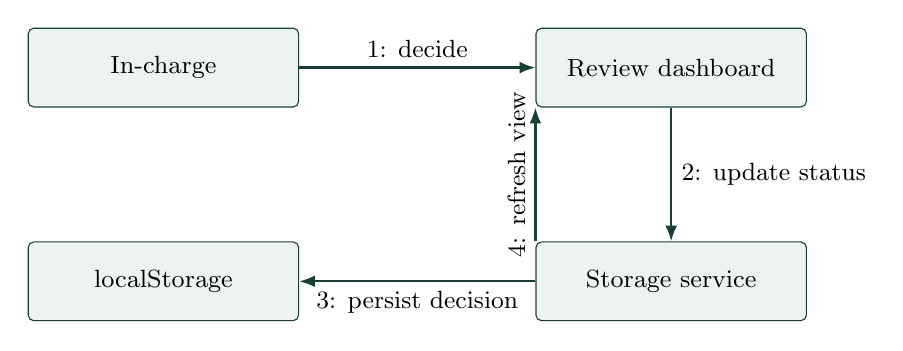
\begin{tikzpicture}[node distance=17mm and 30mm,font=\small]
\node[box](a){In-charge};\node[box,right=of a](b){Review dashboard};
\node[box,below=of b](c){Storage service};\node[box,left=of c](d){localStorage};
\draw[arr](a)--node[above]{1: decide}(b);\draw[arr](b)--node[right]{2: update status}(c);
\draw[arr](c)--node[below]{3: persist decision}(d);
\draw[arr](c.north west)--node[above,sloped]{4: refresh view}(b.south west);
\end{tikzpicture}\caption{Numbered collaboration messages. The storage service also creates the status notification.}
\end{figure}
\clearpage
\section{Conceptual Class and Data Model}
The following model abstracts TypeScript interfaces in \src{src/types/index.ts}. These are data records rather than implemented object-oriented classes or database tables. Identifiers connect records in browser storage, without database-enforced foreign keys.
\begin{figure}[H]\centering
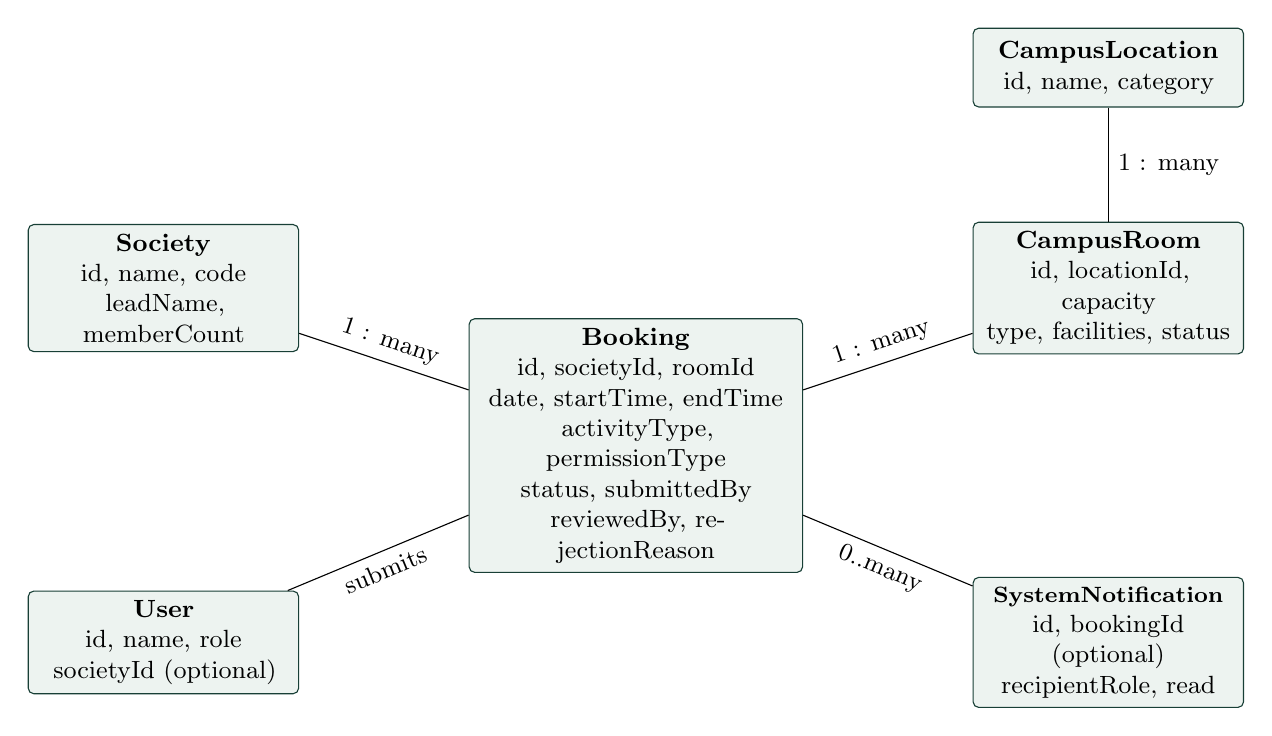
\begin{tikzpicture}[x=1cm,y=1cm]
\node[box,text width=4cm] (b) at (6,0){\textbf{Booking}\\id, societyId, roomId\\date, startTime, endTime\\activityType, permissionType\\status, submittedBy\\reviewedBy, rejectionReason};
\node[box] (s) at (0,2){\textbf{Society}\\id, name, code\\leadName, memberCount};
\node[box] (r) at (12,2){\textbf{CampusRoom}\\id, locationId, capacity\\type, facilities, status};
\node[box] (u) at (0,-2.5){\textbf{User}\\id, name, role\\societyId (optional)};
\node[box] (n) at (12,-2.5){{\footnotesize\textbf{SystemNotification}}\\id, bookingId (optional)\\recipientRole, read};
\node[box] (l) at (12,4.8){\textbf{CampusLocation}\\id, name, category};
\draw (s)--node[above,sloped,font=\small]{1 : many}(b);
\draw (r)--node[above,sloped,font=\small]{1 : many}(b);
\draw (u)--node[below,sloped,font=\small]{submits}(b);
\draw (b)--node[below,sloped,font=\small]{0..many}(n);
\draw (l)--node[right,font=\small]{1 : many}(r);
\end{tikzpicture}\caption{Conceptual relationships derived from source interfaces.}
\end{figure}
\subsection{Reservation Status Model}
\begin{center}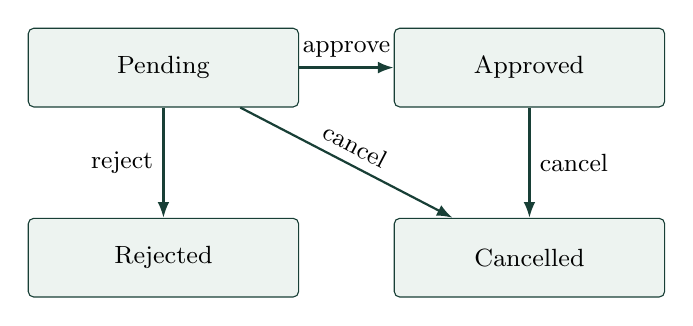
\begin{tikzpicture}[node distance=14mm and 12mm]
\node[box](p){Pending};\node[box,right=of p](a){Approved};\node[box,below=of p](r){Rejected};\node[box,below=of a](c){Cancelled};
\draw[arr](p)--node[above,font=\small]{approve}(a);\draw[arr](p)--node[left,font=\small]{reject}(r);\draw[arr](p)--node[above,sloped,font=\small]{cancel}(c);\draw[arr](a)--node[right,font=\small]{cancel}(c);
\end{tikzpicture}\end{center}
This diagram communicates the intended interface lifecycle. The storage service accepts a status value directly, so production software should enforce allowed transitions and permissions on the server.
\clearpage
\section{Data Flow Diagrams}
\subsection{DFD Level 0: System Context}
\begin{figure}[H]\centering
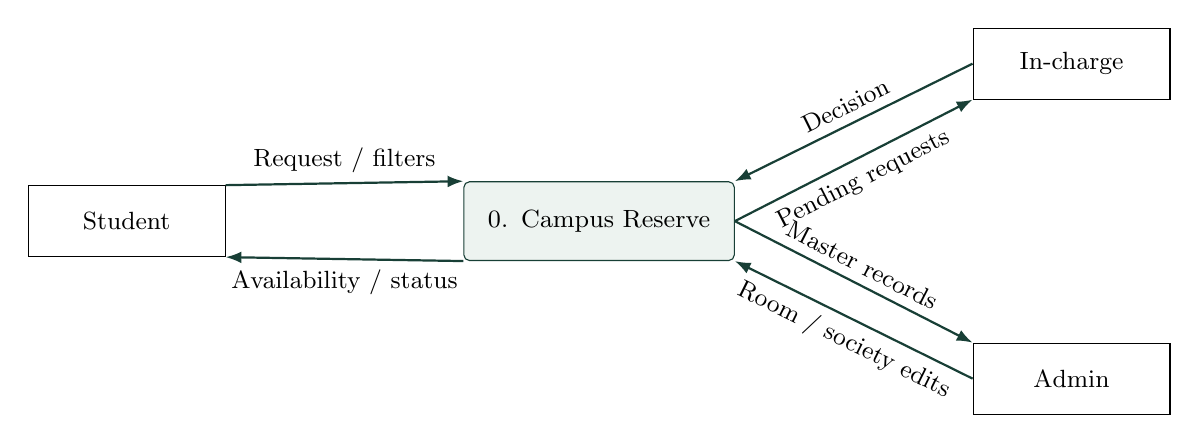
\begin{tikzpicture}[x=1cm,y=1cm,font=\small]
\node[box](p)at(6,0){0. Campus Reserve};\node[actor](s)at(0,0){Student};\node[actor](i)at(12,2){In-charge};\node[actor](a)at(12,-2){Admin};
\draw[arr](s.north east)--node[above]{Request / filters}(p.north west);\draw[arr](p.south west)--node[below]{Availability / status}(s.south east);
\draw[arr](i.west)--node[above,sloped]{Decision}(p.north east);\draw[arr](p.east)--node[below,sloped]{Pending requests}(i.south west);
\draw[arr](a.west)--node[below,sloped]{Room / society edits}(p.south east);\draw[arr](p.east)--node[above,sloped]{Master records}(a.north west);
\end{tikzpicture}\caption{External data exchanges with the browser application.}
\end{figure}
\subsection{DFD Level 1: Core Processes}
\begin{figure}[H]\centering
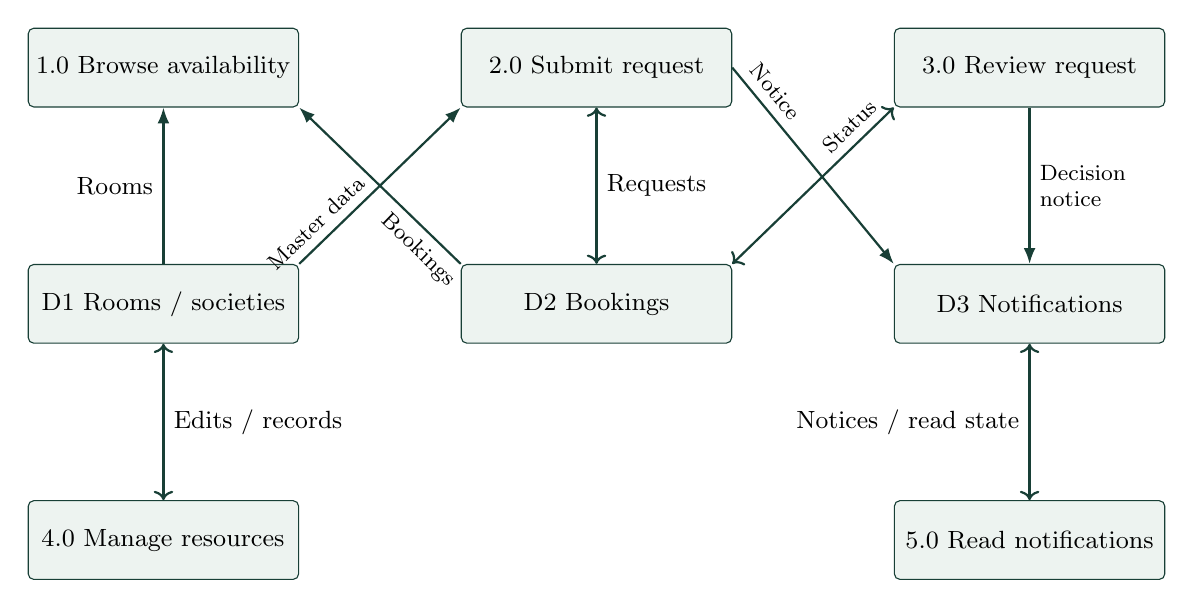
\begin{tikzpicture}[x=1cm,y=1cm,font=\small]
\node[box](p1)at(0,1){1.0 Browse availability};\node[box](p2)at(5.5,1){2.0 Submit request};\node[box](p3)at(11,1){3.0 Review request};
\node[box](d1)at(0,-2){D1 Rooms / societies};\node[box](d2)at(5.5,-2){D2 Bookings};\node[box](d3)at(11,-2){D3 Notifications};
\node[box](p4)at(0,-5){4.0 Manage resources};\node[box](p5)at(11,-5){5.0 Read notifications};
\draw[arr](d1)--node[left]{Rooms}(p1);\draw[arr](d2.north west)--node[pos=.18,below,sloped,font=\footnotesize]{Bookings}(p1.south east);
\draw[arr](d1.north east)--node[pos=.18,above,sloped,font=\footnotesize]{Master data}(p2.south west);\draw[arr,<->](p2)--node[right]{Requests}(d2);
\draw[arr,<->](p3.south west)--node[pos=.2,above,sloped,font=\footnotesize]{Status}(d2.north east);\draw[arr](p2.east)--node[pos=.18,above,sloped,font=\footnotesize]{Notice}(d3.north west);
\draw[arr](p3)--node[right,font=\footnotesize,align=left]{Decision\\notice}(d3);\draw[arr,<->](p4)--node[right]{Edits / records}(d1);\draw[arr,<->](d3)--node[left]{Notices / read state}(p5);
\end{tikzpicture}\caption{Logical decomposition. D1--D3 represent collections in localStorage.}
\end{figure}
The actor exchanges in Level 0 connect to their respective Level 1 processes: students use 1.0, 2.0 and booking tracking; the in-charge uses 3.0; the administrator uses 4.0. Users read notifications through 5.0. Booking tracking reads D2 and cancellation updates D2 through the storage service.
\clearpage
\subsection{DFD Level 2: Reservation Validation}
\begin{figure}[H]\centering
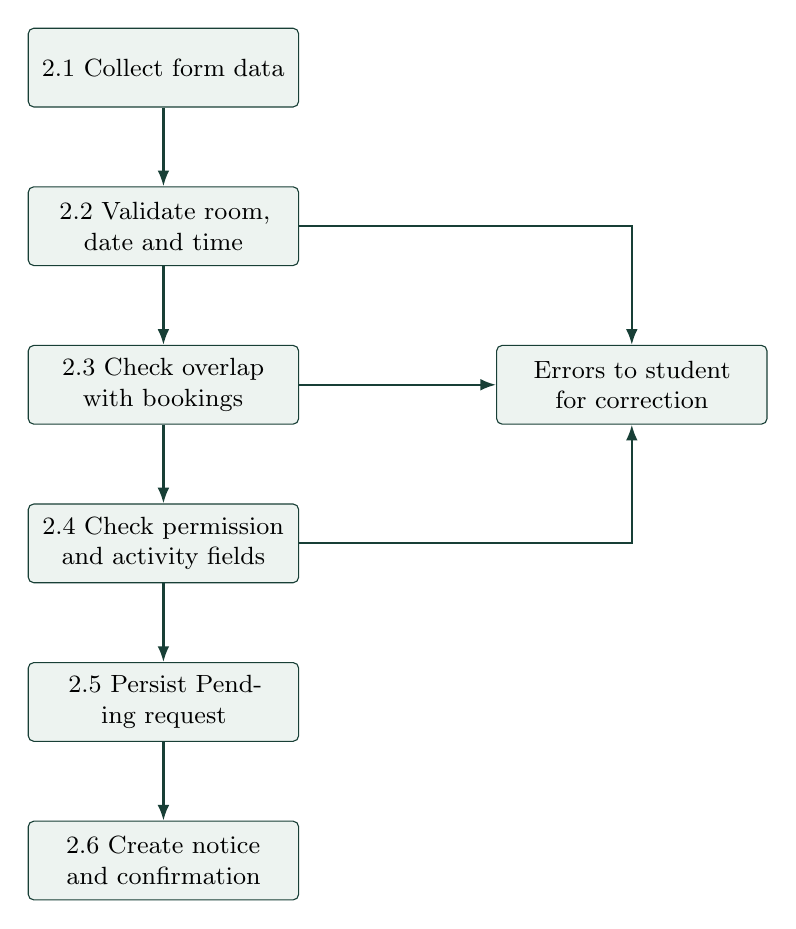
\begin{tikzpicture}[node distance=10mm]
\node[box](a){2.1 Collect form data};\node[box,below=of a](b){2.2 Validate room, date and time};\node[box,below=of b](c){2.3 Check overlap with bookings};\node[box,below=of c](d){2.4 Check permission and activity fields};\node[box,below=of d](e){2.5 Persist Pending request};\node[box,below=of e](f){2.6 Create notice and confirmation};
\foreach \x/\y in {a/b,b/c,c/d,d/e,e/f}{\draw[arr](\x)--(\y);}
\node[box,right=25mm of c](err){Errors to student for correction};
\draw[arr](b.east)-|(err.north);\draw[arr](c.east)--(err.west);\draw[arr](d.east)-|(err.south);
\end{tikzpicture}\caption{Decomposition of request submission. Each failed check prevents progression.}
\end{figure}
\subsection{Conflict Rule and Examples}
For the same room and date, the service identifies overlap when
\[start_{new}<end_{existing}\quad\land\quad end_{new}>start_{existing}.\]
Only Pending and Approved records enter this comparison. The implementation compares normalized time strings in \texttt{HH:mm} format.

\begin{tabularx}{\textwidth}{@{}YYY@{}}\toprule Existing booking & New request & Expected comparison\\\midrule 10:00--11:00, Approved & 10:30--11:30 & Conflict\\10:00--11:00, Pending & 11:00--12:00 & No overlap\\10:00--11:00, Rejected & 10:30--11:30 & Does not block\\\bottomrule\end{tabularx}

These are explanatory examples, not recorded executions. A shared deployment needs an atomic server-side conflict check because separate browser stores cannot coordinate simultaneous users.
\clearpage
\section{Software Requirements Specification}
\subsection{Introduction and Overall Description}
\textbf{Purpose:} specify the behaviour of Campus Reserve for an academic prototype and identify requirements for a future shared service. The audience includes the project team, faculty evaluator and future maintainers.

\textbf{Product perspective:} a browser-based single-page application with seeded demo data and local persistence. React Router maps URLs to pages, AuthContext supplies a demo user, and the storage service handles data reads and writes.

\textbf{User classes:} students submit and track requests, in-charges review them, and administrators maintain master records. These roles describe workflows, not secure authorization guarantees.

\textbf{Operating environment:} a modern browser with JavaScript and localStorage. Development uses Node.js and Vite. The repository README specifies Node.js 22.12 or newer. The campus photograph requires internet access and has a typographic fallback.
\subsection{Functional Requirements}
\begin{longtable}{@{}p{13mm}p{104mm}p{22mm}@{}}\toprule ID & Requirement & Evidence\\\midrule\endhead
FR-01 & The interface shall offer student, in-charge and admin demo personas. & README\\
FR-02 & The schedule shall filter availability by location, room and date. & Schedule view\\
FR-03 & Selecting an hourly slot shall populate the booking form. & Schedule and form\\
FR-04 & The reservation form shall collect activity, society, location, room, time, permission and activity details before review. & Booking form\\
FR-05 & Validation shall reject unavailable rooms, past dates, reversed intervals and overlapping active reservations. & Form, storage service\\
FR-06 & Requests ending after 20:00 shall require Night Permission. & Booking form\\
FR-07 & Submission shall create a Pending booking and an in-charge notification. & Storage service\\
FR-08 & The booking screen shall support search, status filters, details and cancellation. & README\\
FR-09 & The in-charge shall be able to approve or reject requests. & README, review page\\
FR-10 & The admin shall be able to add or update rooms and societies. & README, storage service\\
FR-11 & Notifications shall support persistent read state. & Storage service\\
\bottomrule\end{longtable}
\clearpage
\subsection{Non-functional Requirements and Constraints}
\begin{tabularx}{\textwidth}{@{}p{28mm}YY@{}}\toprule Area & Prototype evidence & Production requirement / target\\\midrule Usability & Responsive navigation, focus styles and dialog handling are documented. & Validate keyboard and mobile journeys with users.\\Security & Passwords are not verified; data is client-controlled. & Verified identity and server-side role/record authorization.\\Consistency & Persistence uses one browser's localStorage. & Shared database and atomic conflict prevention.\\Reliability & Storage failures can be logged by the service. & Surface failed writes and provide backup/recovery.\\Performance & Local filtering and overlap comparisons exist. & Measure response times with representative data and concurrent users.\\Maintainability & Typed records and a central storage service separate concerns. & Preserve interfaces while replacing local storage with an API.\\Privacy & Notifications route by role in the demo. & Deliver messages only to authorized individual recipients.\\\bottomrule\end{tabularx}
No numerical performance target or uptime guarantee has been measured for this report. Such targets should be agreed before a campus pilot.
\subsection{External Interfaces}
\textbf{User interface:} overview, availability schedule, booking wizard, booking list, notification view, in-charge queue and admin management screens.

\textbf{Software interface:} the present application calls a TypeScript storage service and browser APIs. It has no application server API or database connection. The external photograph URL is a display asset, not a booking service.

\textbf{Data interface:} rooms, societies, locations, bookings and notifications serialize as JSON in named localStorage keys. User context provides demo identity information.
\subsection{Acceptance Boundary}
A successful prototype demonstration shows the requested workflow in the same browser. It does not establish secure multi-user deployment, cross-device synchronization or institutional approval authority. Those capabilities require additional implementation and validation.
\clearpage
\section{User Stories and Story Cards}
\begin{tabularx}{\textwidth}{@{}p{13mm}Yp{21mm}@{}}\toprule ID & Story and acceptance criteria & Priority\\\midrule
US-01 & As a society representative, I want to inspect room availability so I can choose a suitable slot.\newline Acceptance: changing location, room or date updates the schedule; selecting a slot carries its details to the form. & High\\
US-02 & As a student, I want to submit a complete reservation so the in-charge can review it.\newline Acceptance: valid submission creates a Pending record with a booking ID. & High\\
US-03 & As a student, I want conflict feedback so I can revise an overlapping request.\newline Acceptance: an overlap with Pending or Approved bookings blocks progression; adjacent intervals do not overlap. & High\\
US-04 & As an in-charge, I want to record a decision so students can see the outcome.\newline Acceptance: the record stores Approved or Rejected with available review details, and a notification is created. & High\\
US-05 & As a student, I want to cancel a booking I no longer need.\newline Acceptance: confirming the offered cancellation action stores Cancelled and updates the view. & Medium\\
US-06 & As an administrator, I want to maintain rooms and societies so the prototype uses current master data.\newline Acceptance: a saved add/edit operation appears in the relevant list. & High\\
US-07 & As a user, I want read-state tracking so I can distinguish new notifications.\newline Acceptance: marking a message read persists after refreshing the same browser. & Medium\\\bottomrule\end{tabularx}
Priorities are proposed for evaluation planning. No velocity or story-point estimates are asserted because a team estimation session was not supplied.
\chapter{Prototype Design and Technology}
\section{Technology Stack}
\begin{tabularx}{\textwidth}{@{}p{35mm}p{27mm}Y@{}}\toprule Technology & Declared version & Role\\\midrule React / React DOM & 19.2.8 range & Component-based interface and rendering\\TypeScript & 6.0.2 range & Typed records and application logic\\Vite & 8.3.0 range & Development server and production build\\React Router DOM & 7.18.3 range & Browser routes and navigation\\Tailwind CSS & 4.3.3 range & Utility CSS and Vite integration\\Lucide React & 1.44.0 range & Interface icons\\Browser localStorage & Browser API & Local JSON persistence\\Oxlint & 1.81.0 range & Static lint tooling\\\bottomrule\end{tabularx}
Versions summarize \src{package.json} declarations, which use caret or tilde ranges. The lockfile determines exact installed versions. The prototype also uses custom CSS in \src{src/design/portal.css}. There is no Node.js backend merely because Node.js runs the build tools.
\section{System Architecture}
\begin{figure}[H]\centering
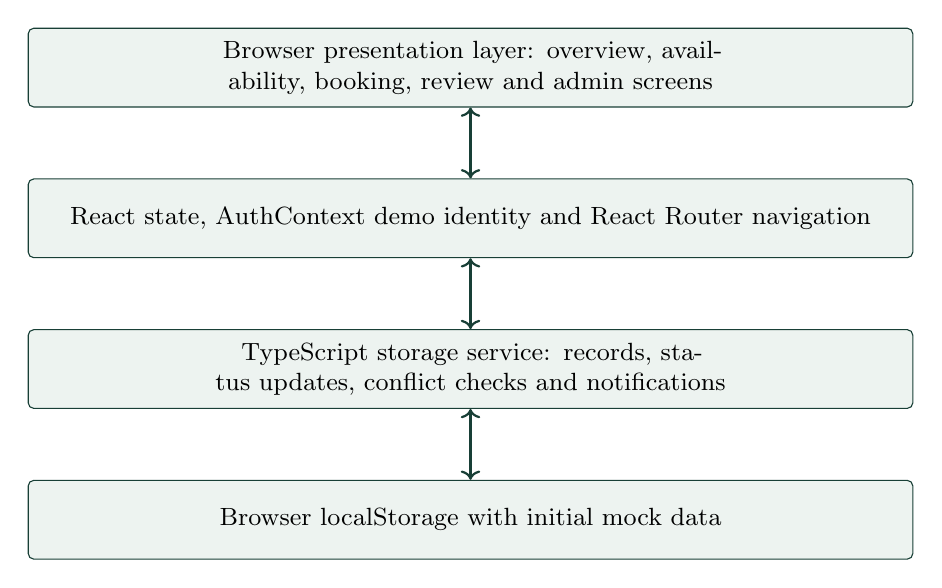
\begin{tikzpicture}[node distance=9mm]
\node[box,text width=11cm](ui){Browser presentation layer: overview, availability, booking, review and admin screens};
\node[box,text width=11cm,below=of ui](state){React state, AuthContext demo identity and React Router navigation};
\node[box,text width=11cm,below=of state](svc){TypeScript storage service: records, status updates, conflict checks and notifications};
\node[box,text width=11cm,below=of svc](data){Browser localStorage with initial mock data};
\draw[arr,<->](ui)--(state);\draw[arr,<->](state)--(svc);\draw[arr,<->](svc)--(data);
\end{tikzpicture}\caption{Current architecture: all application layers execute on the client.}
\end{figure}
\clearpage
\section{Prototype Screens and Navigation}
\begin{tabularx}{\textwidth}{@{}p{37mm}YY@{}}\toprule Screen & Purpose & Route / module\\\midrule Sign-in & Switch demo persona & \src{/login}\\Campus overview & View society booking totals and recent requests & \src{/student/dashboard}\\Availability & Inspect hourly room schedule & \src{/availability}\\Book resource & Complete eight request steps & \src{/student/book}\\My Bookings & Search, inspect and cancel requests & \src{/student/bookings}\\Notifications & View messages and read state & \src{/student/notifications}\\In-charge dashboard & Review pending or all requests & \src{/incharge/dashboard}\\Admin rooms / societies & Maintain master records & \src{/admin/rooms}, \src{/admin/societies}\\\bottomrule\end{tabularx}
\section{Eight-step Booking Prototype}
\begin{enumerate}
\item \textbf{Activity:} Society Preparation, Workshop / Session, or Event.
\item \textbf{Society:} search and select the organizing society.
\item \textbf{Location:} choose the campus building or space category.
\item \textbf{Room:} choose the room and avoid records marked Unavailable.
\item \textbf{Date and time:} supply a valid interval and check for conflicts.
\item \textbf{Permission:} select Morning Permission or Night Permission.
\item \textbf{Details:} complete contextual preparation, workshop or event fields.
\item \textbf{Review:} check the complete request before submission.
\end{enumerate}
\section{Illustrative Demonstration Scenario}
A society representative plans a workshop for a future date. They select an available room and a 14:00--16:00 slot, complete the workshop name, speaker and purpose, and submit the request. The application creates a Pending record. The demonstrator switches to the in-charge persona in the same browser, reviews the request and approves it. Returning to the student persona shows the updated booking and a notification.

Repeat with an overlapping request to demonstrate the conflict message. A request beginning exactly when the existing booking ends illustrates the adjacent-interval rule. These are proposed demonstration inputs, not captured live results or screenshots.
\chapter{Validation and Future Scope}
\section{Acceptance Test Plan}
\begin{longtable}{@{}p{12mm}p{65mm}p{70mm}@{}}\toprule ID & Scenario & Expected result\\\midrule\endhead
T01 & Switch between demo personas. & Home/navigation reflects the selected role.\\
T02 & Select a free availability slot. & Form receives room, date and time.\\
T03 & Complete a valid daytime request. & Pending booking and in-charge notice appear.\\
T04 & Request overlapping Pending / Approved time. & Conflict validation blocks progression.\\
T05 & Start at the existing booking's end time. & Overlap check permits the adjacent interval.\\
T06 & Choose an Unavailable room. & Form requests a different room.\\
T07 & Use a past date or end time before start. & Validation rejects the input.\\
T08 & End after 20:00 with Morning Permission. & Form requires Night Permission.\\
T09 & Approve or reject a Pending request. & Status, review details and notice update.\\
T10 & Confirm an offered cancellation action. & Booking becomes Cancelled.\\
T11 & Add/edit room or society data. & Updated data appears after a same-browser refresh.\\
T12 & Mark notifications as read. & Read state persists locally.\\\bottomrule\end{longtable}
\section{Evidence and Unverified Areas}
The repository README reports a successful production build and 32 smoke checks. This report records that as a repository claim; the application tests were not independently rerun during document preparation. The listed scenarios above are an acceptance plan, not a pass/fail test log.

Before evaluation, the team should run the repository build and smoke command, then demonstrate the complete workflow in a browser. Responsive layout, keyboard behaviour, storage errors and role transitions need direct observation. Production review must additionally examine authorization, concurrent requests and data recovery.
\section{Limitations and Future Scope}
\begin{enumerate}
\item \textbf{Identity and authorization:} add institutional sign-in and server-side enforcement of role and record access.
\item \textbf{Shared persistence:} replace localStorage with a backend API and database for cross-device data.
\item \textbf{Booking consistency:} make conflict checks and writes atomic, and enforce allowed status transitions.
\item \textbf{Notification delivery:} target individual recipients and consider email or campus notification integration.
\item \textbf{Validation and audit:} enforce participant/capacity policies, retain a decision audit trail, and improve error recovery.
\item \textbf{Evaluation:} collect user feedback and measure performance against agreed criteria before deployment.
\end{enumerate}
These items are proposed extensions and must not be presented as existing functionality.
\section{Conclusion}
Campus Reserve demonstrates the core campus booking journey: discover a room, submit a validated request, review the request and track its status. Its separation of screens, typed data and storage operations provides a useful basis for explaining software engineering analysis and prototype design. The current deliverable remains a browser demonstration. A campus-wide service requires secure identity, shared storage and server-enforced booking rules.
\clearpage
\chapter*{References}\addcontentsline{toc}{chapter}{References}
\begin{enumerate}
\item Project repository, accessed 15 September 2026:\par\url{https://github.com/rishitajain7/campus_resource_managment}.
\item Project overview, prototype limitations and documented verification:\par\href{https://github.com/rishitajain7/campus_resource_managment/blob/main/README.md}{README.md}.
\item Declared dependency versions and scripts: \href{https://github.com/rishitajain7/campus_resource_managment/blob/main/package.json}{package.json}.
\item Data records and roles: \href{https://github.com/rishitajain7/campus_resource_managment/blob/main/src/types/index.ts}{TypeScript data interfaces}.
\item Local persistence, overlap detection and notification creation: \href{https://github.com/rishitajain7/campus_resource_managment/blob/main/src/services/storageService.ts}{src/services/storageService.ts}.
\item Screen routing: \href{https://github.com/rishitajain7/campus_resource_managment/blob/main/src/App.tsx}{src/App.tsx}.
\item Request steps and validation: \href{https://github.com/rishitajain7/campus_resource_managment/blob/main/src/pages/BookResourcePage.tsx}{src/pages/BookResourcePage.tsx}, particularly the form state and validation logic.
\item Supplied format reference: \textit{UCS503\_MidSem\_Report\_LaTeX (2).pdf}. Used for academic organization and cover structure only.
\end{enumerate}
\textbf{Repository snapshot:} the inspected main tree resolved to:\par
{\small\src{153cd3a888d48b0fce656e6a1b4ae696a1815efe}}\par
Links above point to the main branch and may change with later edits.
\end{document}
